\chapter{Design basics of laser interferometers for gravitational-wave detection}
I introduce in this chapter some of the basic principles in the
design of sensitive intstruments (and the LIGO detectors in
particular) to set the stage for delving into the details of the
following chapters. I explain why a Fabry-Perot Michelson laser
interferometer 


\section{Signal versus noise}
The factors that must be considered in the design of any detector can
be grouped into two categories: signal and noise. The ability to make
a claim of detection is largely dependent on the magnitude of the
signal to noise ratio (SNR). An SNR of 8 is desired for detection
confidence in LIGO. For laser interferometers, the strength of the GW
signal is proportional to the length of the arms and the amount of
power in the arms. (See Eq. \ref{}.) The change in the distance
between the mirrors, $\Delta L$, is bigger for a given strain the
longer the arms. And with more circulating power, the greater the
amount of power that will show up at the AS port for a given
displacement from the dark fringe. Therefore, the two fundamental ways
to make a GW produce a bigger signal in an interferometer are: 1) make
the arms longer, and 2) increase the circulating power.

No matter how large a signal one might have, it won't be found
confidently, or at all, if there is too much noise. The noise itself
is best grouped into categories of displacement noise and sensing
noise which affect the length of the arms and the measurement of the
signal, respectively. Interferometers for GW detection are plagued
primarily by displacement noise below 70~Hz and sensing noise above
200~Hz.

In the next sections I will describe briefly the specific types of
displacement and sensing noises affecting the sensitivity of laser
interferometers. A summary of the noise budget is shown in
Fig. \ref{fig:NB}. 


\begin{figure}
\begin{centering}
%\includegraphics[width=0.8\textwidth]{figures/.pdf}
\caption[LIGO noise budget]{Noise budget place holder.}
\label{fig:NB}
\end{centering}
\end{figure}


\subsection{Displacement noise} 
ground motion, thermal noise

seismic noise physically displaces the mirrors, resulting in changes in the length
of the arm. 

\subsection{Sensing noise}
stray light, shot noise

Shot noise is a quantum mechanical effect of the detection
of photons which creates uncertainty in the phase of the light, and
therefore the power, at the AS port.




\section{Measuring GW strain with light}
\subsection{Light as a photon} 
Consider two wave packets leaving the beam splitter of a Michelson
interferometer at the same time, each heading down a different arm. If
an appropriately polarized gravitational wave is present, the amount
of time the wave packet takes to travel down a stretched arm and back
is:
\begin{equation}
\label{eq:trt+} 
t_{rt+} = \frac{2 L}{c} \left( 1 + \frac{h_+}{2} \right)
\end{equation}
Likewise, for a compressed arm the roundtrip travel time is:
\begin{equation}
\label{eq:trt-} 
t_{rt-} = \frac{2 L}{c} \left( 1 - \frac{h_+}{2} \right)
\end{equation}
There is a non-zero $2Lh_+/c$ difference in arrival times at the beam splitter, a quantity
one could measure with an accurate stationary clock. This demonstrates intuitively that
a laser interferometer can detect gravitational waves.

It should be noted that we had to use the approximation that the
gravitational wave wavelength $\lambda_{gw}$ is much larger than the
interferometer arm length $L$. This means that the temporal variation
of $h_+(t)$ is negligible during the time it takes the photon to make
its roundtrip. Thus, $h_+$ is treated as a constant in
Eqs. \ref{eq:trt+} and \ref{eq:trt-}.


\subsection{Light as a wave}
The detector at the beam splitter is not a clock, but a photodetector
which is sensitive to phase. It would be informative, therefore, to express
the difference in arrival times as a difference in phase. To do so, we
must move away from the photon model and think about the wave model of
light.  The light wave's phase is given by $\phi = \omega t$ where $t$ is the proper time. Then, the
difference in phase between the two light beams after each has
completed its roundtrip is:
\begin{equation}
\Delta \phi = \phi_{rt+} - \phi_{rt-} = \frac{2 L \omega}{c} h_+
\end{equation}
Two time derivatives yields 
\begin{equation}
\frac{d^2\Delta \phi}{dt^2} = \frac{2 L \omega}{c} \partial_t \partial_t h_+.
\end{equation}
It can be shown \cite{Garfinkle2005Gauge} that the Riemann tensor in
the TT gauge is $R_{tkti}~=-\frac{1}{2}\partial_t \partial_t h_{ki}$,
and gauge invariant. Therefore, our
physically measurable quantity can be expressed as being manifestly
gauge invariant, proving that a laser interferometer can detect the
effect of gravitational waves.






\section{Power-recycled Fabry-Perot Michelson interferometers}
The typical detector configuration is a power-recycled Fabry-Perot
Michelson laser interferometer featuring suspended test masses in
vacuum as depicted in Figure \ref{fig:IFOschematic}. A diode-pumped,
power amplified, and intensity and frequency stabilized Nd:YAG laser
emits light at 1064~nm. The laser is directed to a Michelson
interferometer whose two arm lengths are set to maintain destructive
interference of the recombined light at the anti-symmetric (AS)
port. An appropriately polarized gravitational wave will
differentially change the arm lengths, producing signal at the AS port
proportional to the GW strain and the input power. The Fabry-Perot
cavities in the Michelson arms and a power recycling mirror (RM) at
the symmetric port are two modifications to the Michelson
interferometer that increase the laser power in the arms and therefore
improve the detector's sensitivity to GWs.

\begin{figure}
\begin{centering}
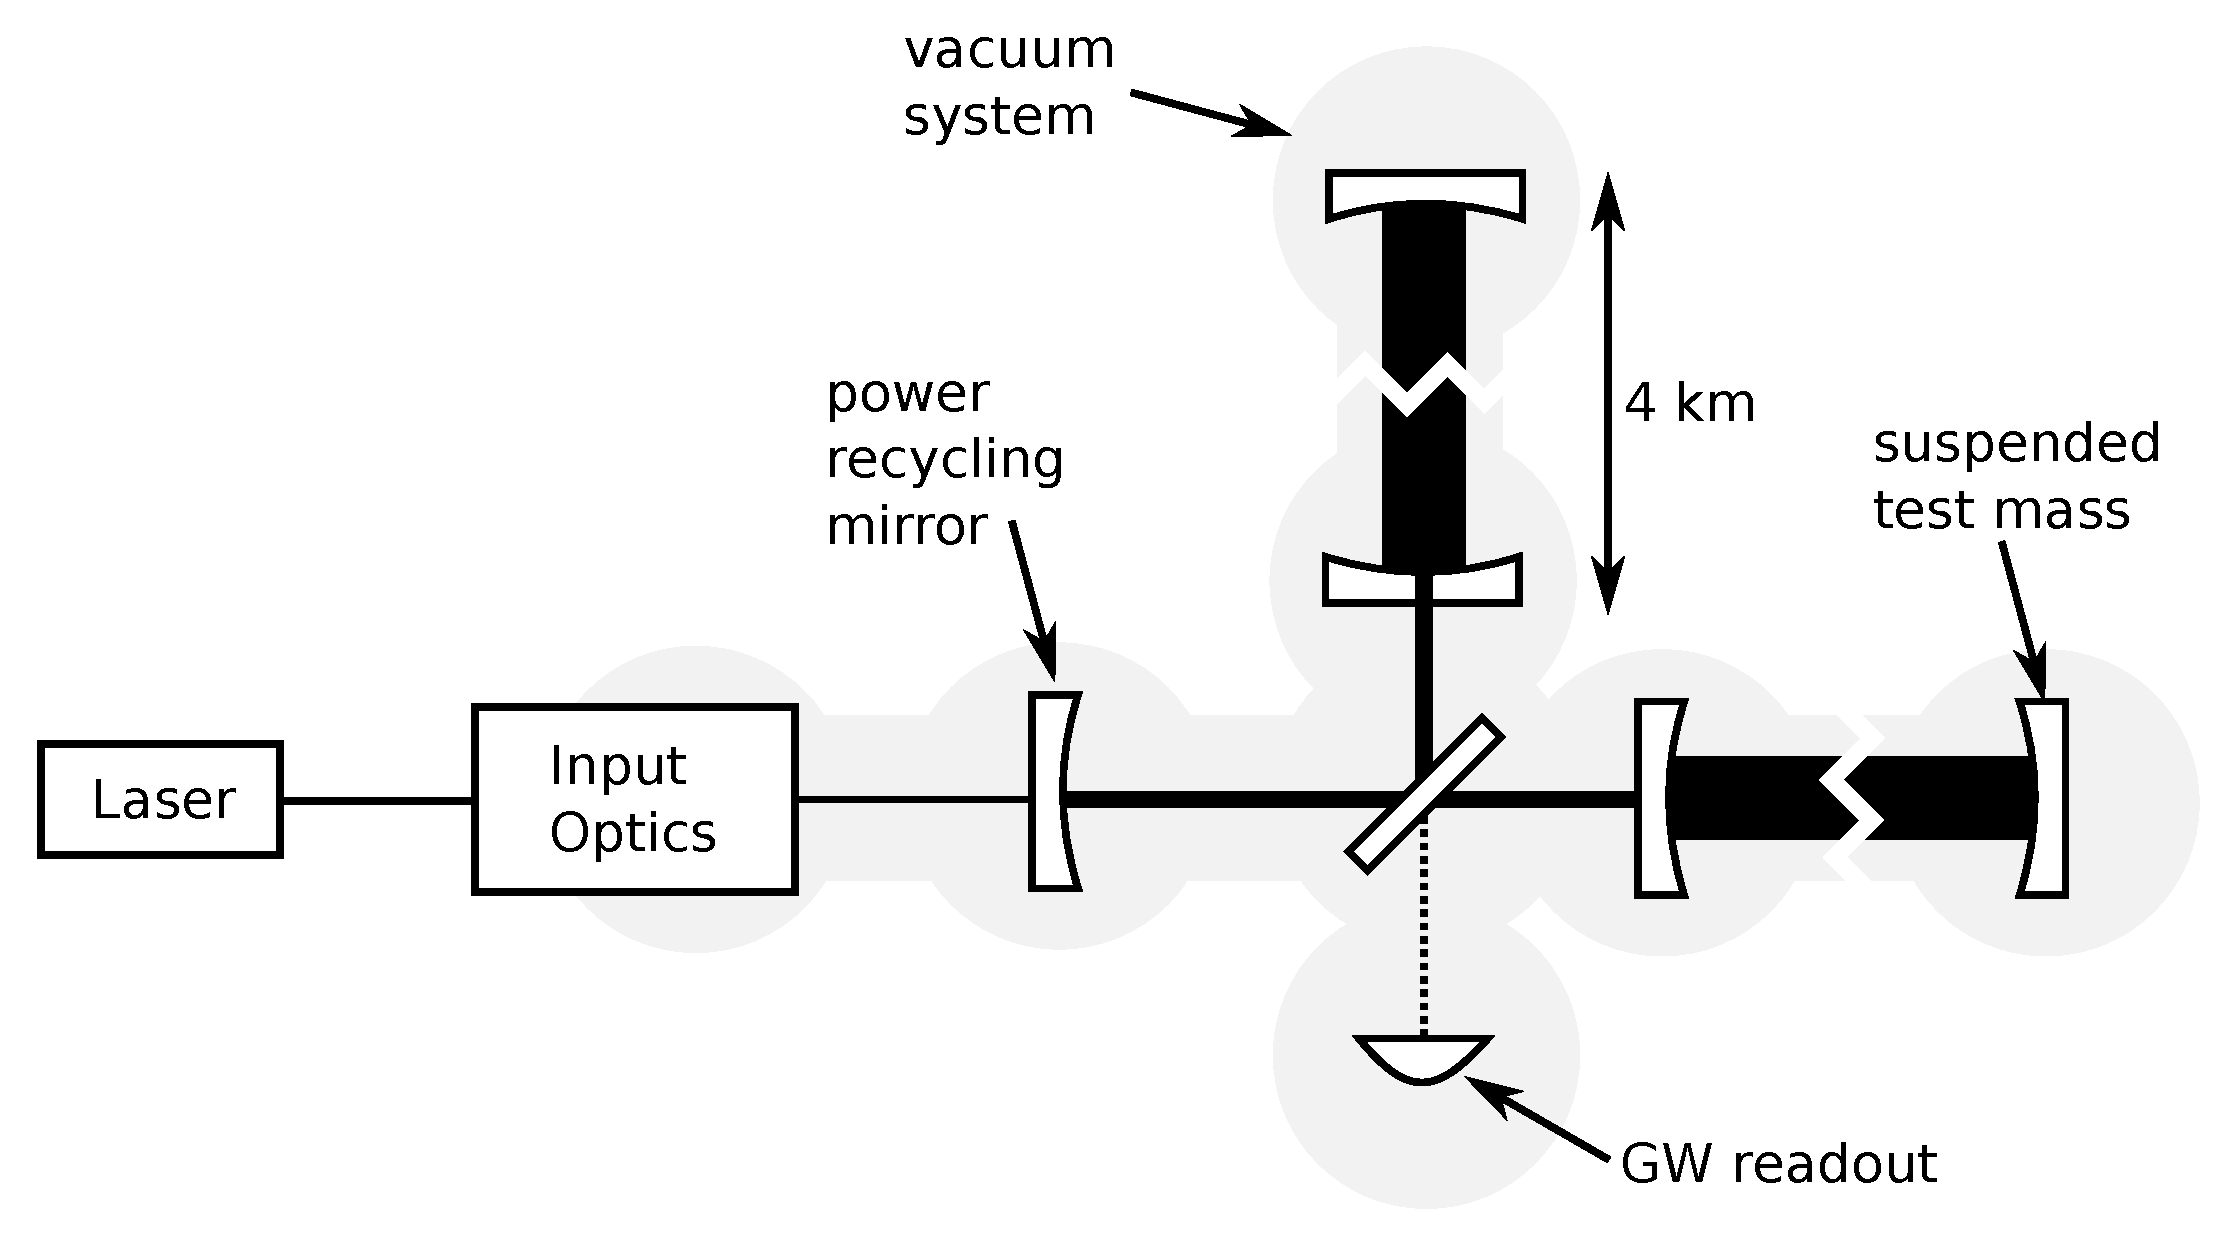
\includegraphics[width=0.8\textwidth]{figures/IFOschematic.pdf}
\caption[Power-recycled Fabry-Perot Michelson laser interferometer]{Power-recycled Fabry-Perot Michelson laser interferometer.}
\label{fig:IFOschematic}
\end{centering}
\end{figure}



\section{Controlling the interferometer}
The ability of the interferometer to provide a differential arm length
signal depends on the many interferometer cavities being locked
\textcolor{blue}{(define locking!)} all at once since it is the light
that serves as our probe of arm length. The motion of the mirrors
without any control is too large for a locked state to naturally
occur. The rms pendular displacement of the mirrors without control is
1 \micron, equivalent to a full laser wavelength. The arm length would
swing from one free spectral range to the next, never staying put long
enough at any particular FSR. 

The motion of the interferometer mirrors must be controlled enough so
that resonance is achieved and error signals fall in a linear
regime. Since the strain sensitivity is determined by mathematically
undoing the (carefully measured) effect of the control system on DARM,
control does not directly improve the strain sensitivity. The purpose
control serves is to make the strain measurement possible. Control,
however, introduces noise so there is a fine balance that must be
found between too much and too little control.

Design considerations for the control loops include how much motion at
what frequencies can be tolerated, and the signal to noise ratio of
the motion sensor.


\subsection{RF sidebands}



\subsection{Digital Control in LIGO}
Although the interferometer is an analog instrument, it is interfaced
through a digital control system. The analog sensor signals are sent
through an analog-to-digital converter (ADC), digitally filtered, and
then sent through a digital-to-analog converter (DAC) before returning
to the interferometer's actuators as control signals. The use of a digital
control system means complex filters can be more easily implemented
than they would with analog electronics, and the potential 

There a select few control systems that remain completely analog, like
the laser intensity stabilization servo (ISS). When the frequencies of
interest extend beyond several tens of thousands of Hz, the use of
computers becomes impractical.




\subsection{Mirror suspension and actuation}
\label{sec:suspension}
The primary interferometer optics are suspended in vacuum so that they
act like free masses at the frequencies in the GW detection band. Each
mirror is hung from a single \textcolor{blue}{xx m diameter} wire that
loops around the bottom of the barrel of the mirror as shown in
Fig. \ref{fig:suspension}. Stand-offs glued just above the mirror's
center of mass on both sides of the barrel mark the final point of
contact of the wire with the mirror, and both ends of the wire are
clamped to the top of a suspension cage.

Each mirror is equipped with four optical sensor and electro-magnetic
(OSEM) actuators for providing control to the mirror. Magnets arranged
to form the four corners of a square are glued on the mirror's back
surface, and the OSEM units envelop them. Length control of the
cavities, for instance, sends current of the same magnitude through
each coil on a given mirror to provide a piston force for changing the
mirror's position.

Minimal contact with the mirrors is necessary to avoid thermal
noise. Therefore, the suspensions provide minimal damping to the
mirrors. Damping for the large optics is instead achieved
electronically through the use of optical levers. Figure
\ref{fig:oplevOLG} shows the open loop gain of the optical lever
servo, demonstrating that it provides velocity damping only (no DC
control) between 0.2~Hz and 2~Hz.

\begin{figure}
\begin{centering}
\subfigure{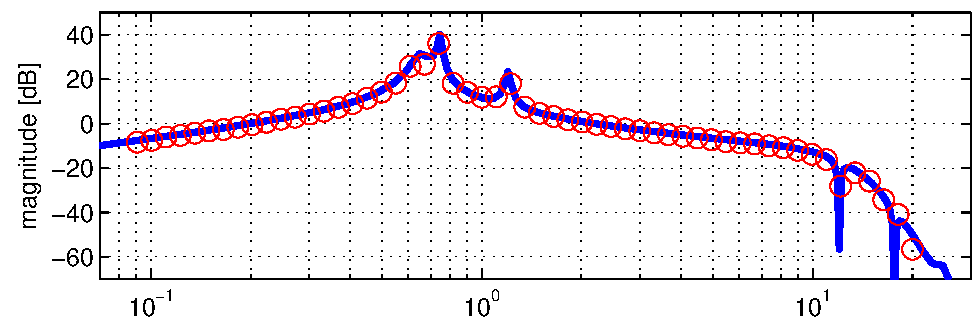
\includegraphics[width=1.0\textwidth]{figures/oplevEX_mags.pdf}}
\subfigure{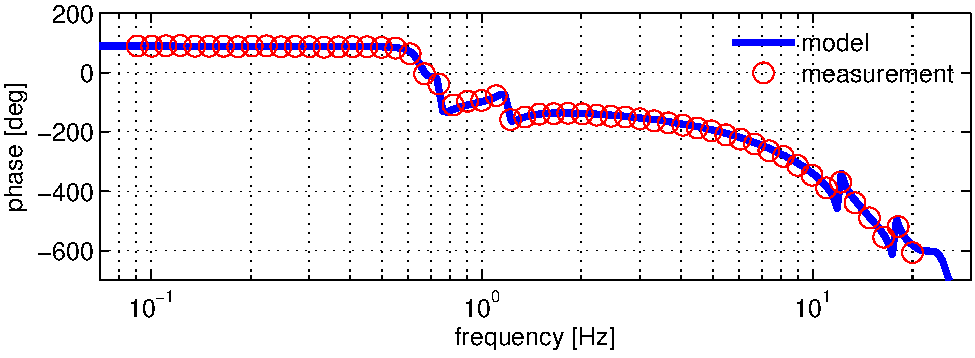
\includegraphics[width=1.0\textwidth]{figures/oplevEX_phases.pdf}}
\caption[Optical lever open loop transfer function]{ETMX pitch optical
  lever open loop transfer function. Uses the filters in the oplev
  servo filter bank, only (no coil output filters). The model of the
  plant is tuned to match the data, resulting in a pitch resonance of
  0.65 Hz and a damping factor of $\gamma$ = 0.02. The UGF is at
  2.2~Hz and the phase margin is $38^\circ$.}
\label{fig:oplevOLG}
\end{centering}
\end{figure}

The suspensions are AC damped at all times for each of the large
optics through optical lever witnesses. Keeping the mirrors quiet
enough with respect to their local ground is necessary to allow for
the initial locking of the interferometer, so each suspended optic,
small and large, is quieted by its OSEM signals during the initial
locking stages. After the interferometer is locked, the angular OSEM
feedback is turned off, and the position OSEM feedback remains.

pitch and yaw



\section{More Laser Power}
Shot noise results from an uncertainty in the arrival time of photons
on a detector:
\begin{equation}
P_{shot} = \sqrt{2 h_p \nu P_{DC}} \mbox{ W/$\sqrt{\mbox{Hz}}$}
\label{eq:shotnoise}
\end{equation}
where $P_{DC}$ is the DC power on the wavefront sensor, $h_p$ is
Planck's constant and $\nu$ is the frequency of the laser light.



